\documentclass[a4paper]{article}
\usepackage[english]{babel}
\usepackage[utf8x]{inputenc}
% package for including graphics with figure-environment
\usepackage{graphicx}
\usepackage{hyperref}
% colors for hyperlinks
% colored borders (false) colored text (true)
\hypersetup{colorlinks=true,citecolor=black,filecolor=black,linkcolor=black,urlcolor=black}

% Commentbox package
\usepackage[most]{tcolorbox}

% package for bibliography
\usepackage[authoryear,round]{natbib}
% package for header
\usepackage[automark,headsepline]{scrlayer-scrpage}
\usepackage{mathtools}
\usepackage{amsmath}
\usepackage{comment}
% qc state brackets
\DeclarePairedDelimiter\bra{\langle}{\rvert}
\DeclarePairedDelimiter\ket{\lvert}{\rangle}
\DeclarePairedDelimiterX\braket[2]{\langle}{\rangle}{#1\,\delimsize\vert\,\mathopen{}#2}

\pagestyle{scrheadings}
\ihead[]{Meyer, Springer, Kawamura, Heidenreich}
\ohead[]{\today}
\cfoot[]{\pagemark} 

\begin{document}
	\title{
	\begin{figure}[!ht]
		% \flushleft
			
\includegraphics[width=0.26\textwidth]{img/THlogoheader.pdf}
	\end{figure}
	\vspace{1cm}
	\Huge Here you can insert the title of \\ your seminar paper \\
	}
	
	\vspace{1cm}
	
	% if you are the only author, you might use the following
	% \author{Name of student}	
	
	% Insert here your name and correct mail address
	\author{\Large \href{mailto:ben_konrad.meyer@smail.th-koeln.de@smail.th-koeln.de}{Ben Konrad Meyer} \and \Large \href{mailto:mike.springer@smail.th-koeln.de}{Mike Springer} \and \Large \href{mailto:kai.kawamura@smail.th-koeln.de}{Kai Kawamura} \and \Large \href{mailto:karl_julian.heidenreich@smail.th-koeln.de}{Julian Heidenreich} \\
	\vspace{1cm}}
	
	% name of the course and module
	\date{
	\large Modul: Verteilte Systeme \\ 
	\vspace{0.8cm}
	\large Lecturer: Name of the lecturer \\
	\vspace{1cm}
	\today
	}

	\maketitle
	\setlength{\parindent}{0pt}

\vspace{2cm}
\begin{abstract}
This template can be used for seminar papers. For more tips and tricks regarding the use of figures, tables, quotations, references, footnotes, enumerations, etc. please download the Masterthesis template. 

\end{abstract}
	\newpage
	\tableofcontents
	\newpage
\section{Introduction} \label{sec:introduction}
The goal of this paper is to explore the opportunities presented by quantum computing and its difficulties,
both in terms of information theoretical Aspects inherent to the concept and in practical aspects of its current
implementations.

Without first introducing the differences between a quantum computer and classical computer most Readers would however
lack the required context to understand the following paper and as such, this introduction will explain the most
critical aspects.

\subsection{Differences between classical and quantum computing theory} \label{subsec:diffclassquanttheory}
The first critical difference between the two computing methods in their theory is their most simple concept of data:
The classical computing theory operates on bits, a simple scalar value that is always one of a finite set of values
(typically either 1 or 0), with their only connection the one imposed by the algorithms in use.
It is also deterministic, with no true randomness, merely internal state that cannot be deduced from outside the system
and can be used to generate unpredictable, but not random values.

In contrast, quantum computing theory operates on the qubit, a superposition of 1 and 0 that is either of the values
with a given probability.
These qubits are typically either represented as a complex number or a unit vector.
Furthermore, for must practical application the qubits in use are not independent but entangled with some number of
other qubits, forming an entangled register, where the superpositions of the individual qubits are connected.
The probabilistic nature of qubits also gives quantum computing access to true randomness without any need for the
complex pseudo random number generators of classical computing.
Indeed, most quantum computing focuses on eliminating the randomness so that the odds of all correct results combined
come as close to 1 as possible, while the likelihood of the other results are reduced to near zero.

Another difference appears due to the physical requirements of superposition: All operations other than measurement on
a quantum computer must be reversible and copying an arbitrary register is impossible\ref{subsec:no-cloning}.
Neither of these restrictions appears for classical computers and as such while there are quantum algorithms where
quantum computers vastly outperform classical computers there are equally classical algorithms where quantum computers
are far less efficient than classical computers, though every classical algorithm has a quantum equivalent % TODO ref or citefor equivalence

\subsection{Practical differences between classical and quantum computers} \label{subsec:diffclassquantpracticey}
Not only are there inherent differences in the practical aspects between classical and quantum computers, there are also
differences induced by the fact that while classical computing has matured over the past decades, quantum computers are
still in the experimental phase.

One aspect where the two paradigms differ is scalability.
While it is possible to simply increase the number of gates of a classical computers, albeit perhaps sacrificing some
performance per gate and latency to heat dissipation concerns, to produce a more powerful classical computer a quantum
computer requires its system to remain in coherence\cite{find explaination}, which makes any scaling of the system a
complex tasks for physicists in addition to making simply connecting two quantum computers into one larger one impossible.

Another aspect is energy efficiency.
For a classical computer every single state needs a gate, whose operation comes with a small, but quickly compounding
cost in heat loss.
Indeed, heat dissipation concerns are the primary limiters for processor size.
While a quantum computer in theory also produces some waste heat per gate, its gates also operate on a superposition on
states and as such could theoretically be far more energy efficient.
In practice this advantage is however entirely counteracted by the fact that current quantum computers require extremely
low temperatures and as such spend most of their energy not on their actual operation, but on the cooling systems they
require to function.
Should a way to keep a quantum computer stable at room temperature be discovered however, quantum computers would easily
change from less to more energy efficient than classical computers.

The final problem that faces quantum computers that is largely solved by classical computers is error correction.
In a classical computer the occasional errors in gate operation, ironically due to quantum mechanical effects, is
corrected by duplicating the calculation and taking a majority vote of the result.
The no-cloning-theorem\ref{subsec:no-cloning} however prevents quantum computers from copying this approach instead
other algorithms have to be used to avoid the final practical superposition differing too much from the theoretical
superposition determined by the intended algorithm. % TODO ref to error correction chapter


\section{No Cloning Theorem} 
\label{sec:no-cloning}

Einer der faszinierendsten Aspekte der Quantenmechanik ist, dass es unmöglich ist
einen beliebigen unbekannten Quantenzustand perfekt zu duplizieren.
Dieses Konzept ist mit dem No-Cloning-Theorem beschrieben, einem grundlegenden Ergebnis der Quanteninformationstheorie.
Das Theorem hat nicht nur tiefgreifende Auswirkungen auf die Quanteninformatik und die Quantenkommunikation,
sondern auch für unser Verständnis der Natur der Information in Quantensystemen.\\

In der klassischen Physik ist die Vervielfältigung von Informationen einfach:
Ein Kopiergerät kann ein Dokument vervielfältigen, ohne das Original zu verändern.
In der Quantenmechanik wird dieser einfache Vorgang jedoch zu einer nicht trivialen und verbotenen Operation.
Das No-Cloning-Theorem besagt, dass es keine universelle Quantenoperation gibt
die eine identische Kopie eines beliebigen unbekannten Quantenzustands erzeugen kann.\\

In diesem Abschnitt werden wir das No-Cloning-Theorem aus verschiedenen Blickwinkeln betrachten, seinen Beweis diskutieren,
seine Konsequenzen untersuchen und verstehen, wie es die Landschaft der Quantentechnologien prägt.

\subsection{Definition}\label{subsec:definition}
Das No-Cloning-Theorem besagt, dass es unmöglich ist, eine identische Kopie eines unbekannten Quantenzustands zu erzeugen.
Mathematisch gesehen gibt es keinen unitären Operator $U$, der die folgende Bedingung erfüllt:
\begin{equation}
    U(\ket{\psi}\otimes\ket{e})=\ket{\psi}\otimes\ket{\psi}\label {eq:cloning_assertion}
\end{equation}
wobei $\ket{\psi}$ ein beliebiger Quantenzustand und $\ket{e}$ in Hilfszustand ist, der überschrieben werden soll.
Diese Gleichung drückt die Idee aus, dass, wenn wir den Operator $U$ auf den Zustand $\ket{\psi}$ anwenden
(kombiniert mit einem Hilfszustand), zwei Kopien des ursprünglichen Zustands entstehen sollten.
Das Theorem sagt uns, dass es für beliebige $\ket{\psi}$ keinen solchen Operator geben kann,
weil sich die Quanteninformation grundlegend von der klassischen Information unterscheidet.
\subsection{Beweis}\label{subsec:proof}
Als grundlegende Schlussfolgerung der Quantenmechanik gibt es mehrere Beweise für dieses Theorem.
Ein solcher Beweis, ein Widerspruchsbeweis, der der Einfachheit halber gewählt wurde, kann wie folgt definiert werden.

Zuerst nehmen wir zwei beliebige Quantenzustände, $\ket{\psi_1}$ und $\ket{\psi_2}$.
Dann werden diese beiden Zustände mit dem Klon operator $U$ geklont, den wir im vorigen Abschnitt definiert haben
und von dem wir für unseren Widerspruchsbeweis nun annehmen, dass er existiert.
\begin{equation}
\begin{split}
    U(\ket{\psi_1} \otimes \ket{e}) = \ket{\psi_1} \otimes \ket{\psi_1}\\
    U(\ket{\psi_2} \otimes \ket{e}) = \ket{\psi_2} \otimes \ket{\psi_2}
\end{split}\label{eq:clone_two_states}
\end{equation}

Mit dieser Information haben wir jetzt zwei Möglichkeiten, das Skalarprodukt von
$\braket{U(\psi_1 \otimes e)}{U(\psi_2 \otimes e)}$ zu schreiben.
Die eine verwendet das Ergebnis der vorherigen Gleichung, während die andere die Tatsache nutzt,
dass Quantenoperationen das Skalarprodukt ihrer Eingaben bewahren\footnote{\cite{segal_postulates_1947}}.

\begin{equation}
\begin{split}
    \braket{U(\psi_1 \otimes e)}{U(\psi_2 \otimes e)} = \braket{\psi_1 \otimes \psi_1}{\psi_2 \otimes \psi_2}\\
    \braket{U(\psi_1 \otimes e)}{U(\psi_2 \otimes e)} = \braket{\psi_1 \otimes e}{\psi_2 \otimes e}
\end{split}\label{eq:two_scalar_products}
\end{equation}

Einfache Ersetzung führt dann zur folgenden Gleichung
\begin{equation}
    \braket{\psi_1 \otimes \psi_1}{\psi_2 \otimes \psi_2} =
    \braket{\psi_1 \otimes e}{\psi_2 \otimes e}
\label{eq:tensor_equals}
\end{equation}

Da Tensor und Skalarprodukte kompatible sind\footnote{\cite{segal_postulates_1947}} simplifiziert das weiter zu:

\begin{equation}
    \braket{\psi_1}{\psi_2}\braket{\psi_1}{\psi_2}=\braket{\psi_1}{\psi_2}\braket{e}{e}
    \label{eq:scalar_equals}
\end{equation}

Und schließlich, weil für jeden Zustand $\ket{e}$ die Gleichung $\braket{e}{e} = 1$ gilt, kommen wir zu dieser Gleichung:

\begin{equation}
    \braket{\psi_1}{\psi_2}^2 = \braket{\psi_1}{\psi_2}
    \label{eq:square_equals_single}
\end{equation}

Es sollte nun offensichtlich sein, dass diese Gleichung nur zwei Lösungen hat:
$\braket{\psi_1}{\psi_2} = 1$ or $\braket{\psi_1}{\psi_2} = 0$.
Die erste Lösung impliziert, dass $\psi_1 = \psi_2$, was für eine allgemeine Klon-Operation nicht hilfreich ist, erlaubt aber eine
Operation, die Kopien eines bestimmten Zustands erzeugt.
Das ist vor allem nützlich um Quantensysteme in einen bekannten Zustand zu initialisieren.
Die zweite Lösung erlaubt zwar, dass sich $\psi_1$ und $\psi_2$ unterscheiden, und ist damit auf den ersten Blick
vielversprechend, verlangt aber immer noch, dass die beiden Zustände orthogonal zueinander sind.
Das ist zwar weniger restriktiv als die erste Lösung, erlaubt aber immer noch nur eine Operation, die eine bestimmte Klasse
von Zuständen kopieren kann, von der alle Mitglieder zueinander orthogonal sind.
Somit ist auch mit dieser Lösung keine allgemeine Klon-Operation möglich.
\subsection{Folgen}\label{subsec:implications}
Das No-Cloning-Theorem hat weitreichende Auswirkungen auf eine Reihe von Gebieten der
Quantenmechanik und Quanteninformatik.

\subsubsection{Quantenkommunikation}
In der klassischen Informationstheorie ist das Kopieren von Daten eine zentrale Technik, um Information zu vervielfältigen und zu übertragen.
Bei klassischen Bits kann man exakt den gleichen Wert duplizieren, indem man eine Kopie eines Bits erstellt.
Im Gegensatz dazu verhindert das No-Cloning-Theorem das Erstellen von exakten Kopien von Quantenbits (Qubits).\\

Das bedeutet, dass im Bereich der Quantenkommunikation, insbesondere bei der Quantenkryptographie, ein Angreifer,
der versucht die Quanteninformation abzufangen oder zu kopieren, in der Regel Fehler einführen wird, die entdeckt werden können.
Dieses Prinzip bildet die Grundlage für Sicherheitsprotokolle wie Quantum Key Distribution (QKD),
bei denen ein Abhörversuch die Übertragung zerstören würde und somit leicht zu erkennen ist.

\subsubsection{Schutz der Quanteninformation}
Da das No-Cloning-Theorem das exakte Kopieren eines unbekannten Zustands verbietet,
wird auch die Quanteninformation von Natur aus gegen bestimmte Arten von Angriffen geschützt.
In klassischen Computersystemen kann ein Angreifer beliebig viele Kopien von Information erstellen,
um sie zu analysieren und gegebenenfalls zu entschlüsseln.
In einem quantenmechanischen System jedoch kann ein Datenexfiltrationsversuch oder das Kopieren eines Zustands
nicht ohne weiteres erfolgen, ohne dass der Versuch des Kopierens den Zustand verändert
und die Quanteninformation damit entwertet wird.\\

Ein gutes Beispiel für diese Art von Sicherheit ist das BB84-Protokoll für Quantenkryptographie.
Bei der Quantenverschlüsselung wird eine Nachricht durch verschränkte Quantenbits übertragen.
Jeder Versuch, die Nachricht zu kopieren oder abzufangen, verändert den Zustand der Qubits und wird vom Empfänger erkannt.

\subsubsection{Design von Algorithmen}

Das No-Cloning-Theorem hat auch tiefgehende Auswirkungen auf das Quantencomputing.
In klassischen Computern ist das Kopieren von Informationen eine grundlegende Technik, die in vielen Algorithmen und Protokollen verwendet wird.
Quantencomputer hingegen können keine exakten Kopien eines Zustands herstellen, was bedeutet,
dass traditionelle Techniken wie fehlerkorrigierende Codes, die in klassischen Computern üblich sind, in der Quantenwelt nicht direkt anwendbar sind.\\

Allerdings existieren spezielle Quantenfehlerkorrekturcodes, die darauf ausgelegt sind, Fehler zu korrigieren,
die durch das Fehlen einer exakten Kopierbarkeit von Quanteninformation entstehen.
Diese Codes erfordern jedoch eine zusätzliche Anzahl von Qubits und eine komplexe Fehlerkorrekturstrategie,
was das Quantencomputing technisch anspruchsvoll macht.
Trotzdem sind Quantenfehlerkorrekturmethoden von entscheidender Bedeutung für die zukünftige Skalierbarkeit
und Zuverlässigkeit von Quantencomputern und werden später in diesem Artikel genauer beschrieben[\ref{sub:quantum_error_correction}].

\begin{tcolorbox}[title=Kommentar,
    title filled=false,
    colback=cyan!5!white,
    colframe=cyan!75!black]
Verschiedene Messmethoden
Jeder Quantenalgorithmus ist auch grundsätzlich anders als ein klassischer Algorithmus, da Operationen anders implementiert
werden müssen, auch wenn die Theorie des Algorithmus identisch zu einem klassischen Algorithmus ist.
    Dieser Aspekt wird hier allerdings nicht näher behandelt werden.
\end{tcolorbox}

\subsubsection{Speicherung von Quanteninformation}
Das No-Cloning-Theorem hat weitreichende Konsequenzen für die Quanteninformationstheorie,
insbesondere für die Konzepte der Informationsspeicherung und -übertragung.
Die Unmöglichkeit des Klonens ist eng mit den grundlegenden Prinzipien der Quantenmechanik wie Überlagerung und Verschränkung verknüpft.
Sie hindert die Schaffung von perfekten Kopien von Quanteninformation und erfordert, dass Information auf neue, kreative Weise verarbeitet und gespeichert wird.\\

Ein interessantes Beispiel sind die Quantenlogikgatter, die in Quantencomputern verwendet werden.
Diese Gatter müssen mit den Einschränkungen des No-Cloning-Theorems arbeiten und können keine klassischen,
deterministischen Kopien erzeugen, sondern müssen die Quanteninformation in verschränkten oder überlagerten Zuständen manipulieren.

\subsubsection{Messungen und Messgenauigkeit}

In der Quantenmetrologie, die sich mit der präzisen Messung von quantenmechanischen Systemen beschäftigt,
beeinflusst das No-Cloning-Theorem ebenfalls die Art und Weise, wie Messungen durchgeführt werden können.
Da das exakte Kopieren von Zuständen nicht möglich ist, kann das Präzisionsmaß für Messungen nicht durch das
Vervielfachen von Messinstrumenten oder durch das Erstellen von Kopien von Quantenobjekten verbessert werden.
Stattdessen wird die Quantenmessung durch andere Techniken wie
Quanteninterferometrie und den Einsatz von verschränkten Zuständen optimiert.




\section{Quantenteleportation}\label{sec:quantum-teleportation}

\subsection{Einführung}\label{subsec:introduction}
Quantenteleportation ist ein bahnbrechendes Phänomen, das die Übertragung von Quanteninformationen
zwischen zwei entfernten Orten ermöglicht, ohne dass das Teilchen oder Objekt, das die Information trägt, physisch bewegt wird.
Im Gegensatz zur theoretischen klassischen Teleportation, bei der es um den Transport von Materie oder Energie geht,
konzentriert sich die Quantenteleportation auf die Übertragung von Quantenzuständen.
Dieser Prozess nutzt die Prinzipien der Quantenmechanik, einschließlich Verschränkung, Superposition,
und das No-Cloning-Theorem,
um den Zustand eines Quantenobjekts (z.B.\ eines Photons oder eines Elektrons) von einem Ort zum anderen zu übertragen.
Dabei spielt die Entfernung der Objekte keine Rolle.\\

Der Begriff ``Quantenteleportation'' kann etwas irreführend sein, da bei diesem Prozess keine eigentliche Materie teleportiert wird.
Was stattdessen ``teleportiert'' wird, ist die Information über den Quantenzustand eines Teilchens.
Der Schlüssel zur Quantenteleportation ist die Quantenverschränkung,
ein Phänomen, bei dem zwei oder mehr Teilchen so miteinander korrelieren, dass der Zustand des einen Teilchens den Zustand des anderen augenblicklich
 beeinflusst, unabhängig davon, wie weit sie voneinander entfernt sind.
Diese ``gespenstische Fernwirkung'', wie Albert Einstein sie nannte,
ermöglicht die Übertragung von Quanteninformation zwischen weit entfernten Parteien, ohne dass die oft fragilen Quantenzustände selbst transportiert werden müssen.

\subsection{Aufbau}\label{subsec:setup}

Es muss ein Quanten-Verschränkungspaar vorhanden sein.
Dieses Paar muss sich im Bell-Zustand\cite{quantuminfocambridge} befinden, um sicherzustellen, dass die Messung des einen den Zustand des anderen beeinflusst.
Dieses Paar wird in der Regel durch einen Prozess wie
Spontane parametrische Abwärtsumwandlung\cite{couteau2018spontaneous} erzeugt.
Derzeit werden dafür in der Regel einfache Photonen oder Ionen verwendet.\\


Außerdem müssen sich an den Endpunkten der Teleportation zwei Parteien befinden, im Folgenden Alice und Bob genannt, die beide in der Lage sind, mit Quantensystemen zu interagieren und Messungen vorzunehmen, was normalerweise einen Quantencomputer mit begrenzter Funktionalität bedeutet.
Schließlich muss ein klassischer Kommunikationskanal zwischen Alice und Bob bestehen.
Der Schlüssel für die Quantenteleportation ist hier, dass dieser Kanal nicht in der Lage sein muss, Quantenzustände zu transportieren - dafür ist die Teleportation gedacht -, sondern nur herkömmliche Bits.

%<Diagramm Aufbau>

\subsection{Vorgang}\label{subsec:process}

Nachdem der Aufbau abgeschlossen ist, stellt sich nun die Frage, was tatsächlich getan werden muss, um die Quantenteleportation durchzuführen.
Dies kann in mehrere Schritte aufgeteilt werden.

\subsubsection{Alices Bell Zustand Messung}
Der erste Schritt, den Alice durchführt, ist die Bell-State-Messung, die zwei wichtige Teilschritte umfasst.

Zunächst kombiniert Alice das Teilchen, das sie teleportieren möchte, mit ihrer Hälfte des verschränkten Paares.
Dies geschieht in der Regel mithilfe eines Strahlenteilers oder eines Interferometers, um die beiden Teilchen in einen Superpositionszustand zu versetzen.

Zweitens misst Alice die beiden kombinierten Teilchen in der Bell-Basis, die die Teilchen aus ihren vier möglichen Zuständen in einen einzigen zusammenfallen lässt.
Diese Messung ist entscheidend, denn sie bestimmt, wie Bob sein Teilchen anpassen muss, um den Zustand wiederherzustellen, den
Alice teleportiert.
\subsubsection{Klassische Kommunikation}
Als Nächstes verwendet Alice ihren klassischen Kommunikationskanal, um ihre Messung an Bob zu senden.
Dies erfordert die Übertragung von nur zwei Bits (den beobachteten Zustand des zu teleportierenden Qubits und den beobachteten Zustand des
des verschränkten Paares), was für keinen Kommunikationskanal ein Problem darstellen sollte.
Diese geringe Bandbreitenanforderung in der klassischen Kommunikation macht in der Tat mehrere Kommunikationskanäle verfügbar
die normalerweise wegen ihrer geringen Bandbreite nicht infrage kämen, insbesondere wenn die Teleportation über große
Entfernungen stattfinden soll.
Diese Information reicht jedoch aus, um Bob zu instruieren, wie er sein eigenes System einstellen muss.
\subsubsection{Bobs Quantenoperation}
Nun, da Bob die klassische Messung erhalten hat, muss er eine oder beide (je nach Messung) der folgenden Methoden anwenden: Das
Pauli-X-Gatter für einen Bit-Flip oder das Pauli-Z-Gatter für einen Phasen-Flip.
Durch diese Operation wird sein Quantenzustand in denselben Zustand versetzt, den Alices Quantenteilchen hatten, bevor ihre
Messung die Superposition kollabierte.
Hier ist auch noch einmal darauf hinzuweisen, dass Bob den Zustand erst erstellt, nachdem Alice ihn mit der Messung
bereits zerstört hat - wie das No-Cloning-Theorem besagt\ref{sec:no-cloning} wird der Zustand nie kopiert, sondern nur
übertragen.

Sobald Bob dies getan hat, ist die Quantenteleportation abgeschlossen.
\subsection{Mathematik}\label{subsec:proof2}

\subsubsection{Verschränkung und Bell-Zustände}

Zu Beginn des Prozesses haben wir zwei Teilchen (Teilchen 2 und 3), die sich an den Orten A und B befinden.
Diese Teilchen werden in einem verschränkten Zustand (Bell-Zustand) erzeugt.
Ein Bell-Zustand ist eine der vier möglichen maximal verschränkten Zustände, die ein Paar von Quantenobjekten haben kann.
Ein Beispiel für einen solchen Zustand ist:

\begin{equation}
|\Phi^+\rangle = \frac{1}{\sqrt{2}} \left( |00\rangle + |11\rangle \right)
\end{equation}

Dieser Zustand wird zwischen den beiden Teilchen 2 und 3 geteilt, wobei Teilchen 2 bei A und Teilchen 3 bei B ist.

\subsubsection{Der zu teleportierende Zustand}

Nun nehmen wir an, dass wir den Zustand eines dritten Teilchens (Teilchen 1) teleportieren möchten, das sich am Ort A befindet. Der Zustand des Teilchens 1 kann allgemein als:

\[
|\psi\rangle_1 = \alpha |0\rangle + \beta |1\rangle
\]

ausgedrückt werden, wobei \(\alpha\) und \(\beta\) komplexe Zahlen sind, die den Zustand beschreiben.

\subsubsection{Verschränkung und Messung}

Der gesamte Zustand des Systems (Teilchen 1, 2 und 3) kann als Produktzustand von Teilchen 1 und dem verschränkten Zustand von Teilchen 2 und 3 beschrieben werden:

\[
|\Psi\rangle_{123} = |\psi\rangle_1 \otimes |\Phi^+\rangle_{23} = \frac{1}{\sqrt{2}} \left( \alpha |0\rangle_1 + \beta |1\rangle_1 \right) \otimes \left( |00\rangle_{23} + |11\rangle_{23} \right)
\]

Durch Anwenden der Distributivität ergibt sich:

\begin{gather*}
    |\Psi\rangle_{123} = \frac{1}{\sqrt{2}} \left( \alpha |0\rangle_1 \otimes (|00\rangle_{23} + |11\rangle_{23}) + \beta |1\rangle_1 \otimes (|00\rangle_{23} + |11\rangle_{23}) \right)\\
    |\Psi\rangle_{123} = \frac{1}{\sqrt{2}} \left( \alpha |000\rangle_{123} + \alpha |011\rangle_{123} + \beta |100\rangle_{123} + \beta |111\rangle_{123} \right)\\
\end{gather*}

Nun wird eine Bell-Zustandsmessung auf den Teilchen 1 und 2 durchgeführt, die den Zustand des Systems in einen der vier Bell-Zustände projiziert. Die Messung ist zufällig, und die Ergebnisse können durch die folgenden Zustände beschrieben werden:

\[
|\Phi^+\rangle_{12}, |\Phi^-\rangle_{12}, |\Psi^+\rangle_{12}, |\Psi^-\rangle_{12}
\]

\subsubsection*{Klassische Kommunikation und Zustandserstellung}

Nachdem die Messung durchgeführt wurde, sendet der Ort A das Messresultat an Ort B über einen klassischen Kanal.
Anhand der Nachricht kann Ort B den Zustand des Teilchens 3 (das ursprünglich am Ort B war) in den gewünschten Zustand \(|\psi\rangle_1\) transformieren. Dazu wird eine der folgenden Operationen durchgeführt, abhängig von der Messung, die an Ort A durchgeführt wurde:

\begin{gather*}
    |0\rangle_3 \quad \text{(falls Messung das Ergebnis } |\Phi^+\rangle\text{ ergibt)}\\
    X|0\rangle_3 \quad \text{(falls Messung das Ergebnis } |\Phi^-\rangle\text{ ergibt)}\\
    Z|0\rangle_3 \quad \text{(falls Messung das Ergebnis } |\Psi^+\rangle\text{ ergibt)}\\
    XZ|0\rangle_3 \quad \text{(falls Messung das Ergebnis } |\Psi^-\rangle\text{ ergibt)}\\
\end{gather*}

Durch diese Operationen wird der Zustand des Teilchens 3 in den ursprünglichen Zustand von Teilchen 1 (\( \alpha |0\rangle + \beta |1\rangle \)) überführt.


\subsection{Herausforderungen}\label{subsec:challenges}
Obwohl die Quantenteleportation ein vielversprechender Forschungszweig ist, gibt es noch einige Herausforderungen zu bewältigen

\subsubsection{Verschränkung Erzeugen und Erhalten}
Eine der größten Herausforderung ist die Erzeugung und Erhaltung eines verschränkten Systems zwischen dem Start- und Zielpunkt
der Teleportation.
Die Teleportation ist zwar theoretisch nicht durch Entfernung begrenzt, aber je größer die Entfernung zwischen den Orten
des do schwieriger ist es die verschränkten Teilchen aufzuteilen, ohne die Verschränkung zu beschädigen.\\

Ein Lösungsansatz sind hier Quantenrepeater: Spezialisierte Geräte die die Entfernung zwischen direkt verschränkten Teilchen reduzieren,
indem sie diese nur zwischen Repeater Stationen aufteilen müssen.
In der Station werden dann mithilfe von Entanglement Swapping zwei Verbindungen des Repeaters verschränkt.

\subsubsection{Klassische Kommunikation}
Auch wenn die benötigte Bandbreite der klassischen Kommunikation minimal ist, muss trotzdem ein Kommunikationskanal
existieren.
Das hat zwei signifikante Nachteile: Zum einen ist die klassische Kommunikation auf die Lichtgeschwindigkeit begrenzt,
was ein Geschwindigkeitslimit für die Teleportation erzeugt, auch wenn die ``spukhafte Fernwirkung'' der Quantenmechanik
schneller passieren könnte\cite{hensen2015loophole}.
Zum anderen sind klassische Kommunikationskanäle anfällig für Observation - ein Angreifer kann zwar
ohne das verschränkte Teilchen den Quantenzustand nicht reproduzieren ist aber in der Lage festzustellen, dass die
Kommunikation stattgefunden hat.
Ebenfalls könnte der Angreifer auch die Kommunikation stören, was zwar bei geeigneten Protokollen den Teilnehmern
offensichtlich ist aber trotzdem eine Schwachstelle darstellt.
Die einzige bekannte Lösung ist hier ein robustes klassisches Kommunikationssystem, was für andere Kommunikationszwecke
bereits aufgebaut ist oder wird, aber leider die Lichtgeschwindigkeitslimitation nicht umgehen kann.


\subsubsection{Skalierbarkeit}

Ein weiteres bedeutendes Problem der Quantenteleportation ist die Skalierbarkeit.
Während die Quantenteleportation in kleinen, kontrollierten Systemen von einigen wenigen Qubits relativ einfach durchgeführt werden kann,
stellt die Skalierung auf größere Netzwerke und damit nützliche Datenmengen und die Integration in reale Kommunikationssysteme eine enorme Herausforderung dar.
Um Quantenteleportation praktisch nutzen zu können würde es ein großflächiges System von Kommunikationskomponenten
benötigen.
Die Erstellung dieser bräuchte Quantentechnologien in einer Menge in der diese momentan weder technisch möglich
noch finanziell tragbar ist, wenn man bestehende Preise hochrechnet.\\

Hier ist allerdings die Erwartung, dass weitere Forschung dieses Problem beheben wird.
Es wird sowohl an günstigeren Methoden zur Erstellung von verschränkten Systemen und der Stabilisierung dieser,
als auch an der Erstellung von Quantenkomponenten rege geforscht.
Auch an Forschungsbudget fehlt es hier nicht, da einige große Technologiefirmen wie Google und Microsoft an Quantentechnologie forschen.

\subsubsection{Fehlerquellen und Messgenauigkeit}
Die Messgenauigkeit ist entscheidend für die erfolgreiche Durchführung der Quantenteleportation.
Eine fehlerhafte Messung der Bell-Zustände kann dazu führen, dass der teleportierte Zustand nicht korrekt wiederhergestellt werden kann.
Fehlerquellen können in den Messinstrumenten, in der Kommunikation oder auch in der Quantenverschränkung selbst liegen.

Auch hier wird rege geforscht, da alle drei Aspekte nicht eigen zur Quantenteleportation sind, sondern nahezu alle
Quantenoperationen betreffen.




\section{Quantenhardware}
\label{sec:quantenhardware}

Die Realisierung eines Quantencomputers ist durch hohe technische herausforderungen geprägt. Um die besonderen Eigenschaften der Qubits eines Quantencomputers, wie Superposition und Verschränkung, nutzen zu können, müssen sie durch externe Einflüsse geschützt werden und die Dekoheränz minimiert werden.
Äußere Einflüsse wie Temperaturschwankungen, elektromagnetische Felder oder Strahlung aller Art können die Qubits beeinflussen. Aus diesem Grund werden Quantencomputer bei extrem niedrigen Temperaturen und in einem Vakuum betrieben.\\

Außerdem ist nicht nur die Herstellung der Qubits eine Herausforderung, sondern auch die Steuerung, Auslesung und Korrektheit von physikalischen Qubits.

\subsection{Dekohärenz}
\label{sub:dekohaerenz}
Dekoheränz ist ein zentrales Konzept, welches wichtig in der Entwicklung von Quantencomputern ist. Der Prozess der Dekoheränz beschreibt den Verlust der koheränten Quanteneigentschaften eines Qubits durch Wechselwirkung mit der Umgebung.
Diese Veränderung führt zu einem Übergang von quantenmechanischem Verhalten zu einem klassischem Verhalten von Bits.\\

In der Quantenmechanik können Systeme in Überlagerungszuständen existieren, wobei mehrere Zustände gleichzeitig eingenommen werden können. Diese Eigenschaft erklärt auch das Phänomen der Quanteninterferenz.
Äußere Einflüsse durch die Umgebung kann eine Verschränkung von Qubits zerstören. Dies führt dazu, dass die Phasenbeziehungen zwischen den Qubits beeinflusst oder gar aufgehoben werden.
Folgernd verliert das System die Interferenzeffekte und verhält sich zunehmend klassischer. Diese Zeit nennt man Dekoheränzzeit.\\

Die \textbf{Dekoheränzzeit} ($T_2$) eines Qubits misst die Länge der Zeit, in der er in der Lage bleibt kohärent zu bleiben, welcher danach von äußeren Einflüssen zerstört wird.
Neben $T_2$ wird auch häufig die \textbf{Relaxationszeit} ($T_1$) gemessen, welche angibt, wie lange ein Qbit im angeregten Zustand bleibt, bevor es auf sein Grundzustand zurückfällt.
In der Realität ist die Dekoheränzzeit jedoch in den meisten Fällen kürzer als die Relaxationszeit.\\

\textbf{Berechnung der Dekoheränzzeit}\\
Durch eine Messung der zeitlichen Abnahme der Koheränz eines beispielhaften Qubits kann die Dekoheränzzeit eines Systems festgelegt werden.
Bei einem Quantencomputer, der auf dem Spin eines Teilchen beruht, kann dies durch die \textbf{Spin-Echo-Methode} gemessen werden.
Quantencomputer, die auf anderen Qubits basieren, haben equivalente Methoden um die Kohärenz zu messen.\\

Das einfachste Modell zur Beschreibung der Dekoheränzzeit ist die \textbf{Exponentielle Abnahme der Kohärenz}

\begin{equation}
    C(t) = C(0)*e^{-t/T_2}
\end{equation}

Dabei ist:\\
$C(t)$ Die Kohärenz des Qubits zum Zeitpunkt t\\
$C(0)$ Die initiale Koheränz\\
$T_2$ Die Dekoheränzzeit\\

Indem man den Kohärenzverlust experimentell misst und die Werte in eine exponentielle Abklingfunktion einpasst, erhält man $T_2$\\

\begin{tcolorbox}[title=Kommentar,
    title filled=false,
    colback=cyan!5!white,
    colframe=cyan!75!black]
    Die \textbf{Dekoheränzzeit} kann auch durch genauere jedoch auch deutlich kompliziertere weise errechnet werden.
    Bekannte Methoden hierfür wären zum Beispiel die Spektrale Analyse, Dynamische Entkopplung, Hahn-Echo und Ramsey-Interferometrie.
    Außerdem wird duch das häufige messen der Dekoheränzzeit diese indirekt verlänger. Diesen Effekt nennt man Quanten-Zeno-Effekt.\\
    Zuletzt muss auch die Lindblad-Gleichung genannt werden welche den Zeitverlauf der Dichtematrix in einem Offenen Quantensystem beschreibt.
    \begin{equation}
        \frac{dp}{dt} = -i[H,p]+\sum_i(L_ipL^\dagger_i-\frac{1}{2}\{L^\dagger_i L_i,p\})
    \end{equation}
    Diese Themen sprengen jedoch den Rahmen dieser Arbeit in Richtung Physik und werden deswegen nicht weiter behandelt.
\end{tcolorbox}

\subsection{Universelle Quantencomputer}
\label{sub:universelle_quantencomputer}
Universelle Quantencomputer beruhen grundlegend auf einem Gatter Modell, wie bereits in diesem Artikel beschrieben. Folgend sind drei der meist erforschten
Methoden, welche dieses Modell physikalisch umsetzen.\\

Ein prominentes Beispiel für die Umsetzung eines universellen Quantencomputers ist der \textbf{Sycamore Chip}, welcher auf supraleitenden Qubits basiert.
Dieser Chip ist in einem Gatter angeordnet für die Kommunikation zwischen Qubits und die durchführung von Quantenoperationen.\\

\begin{figure}[H]
    \centering
    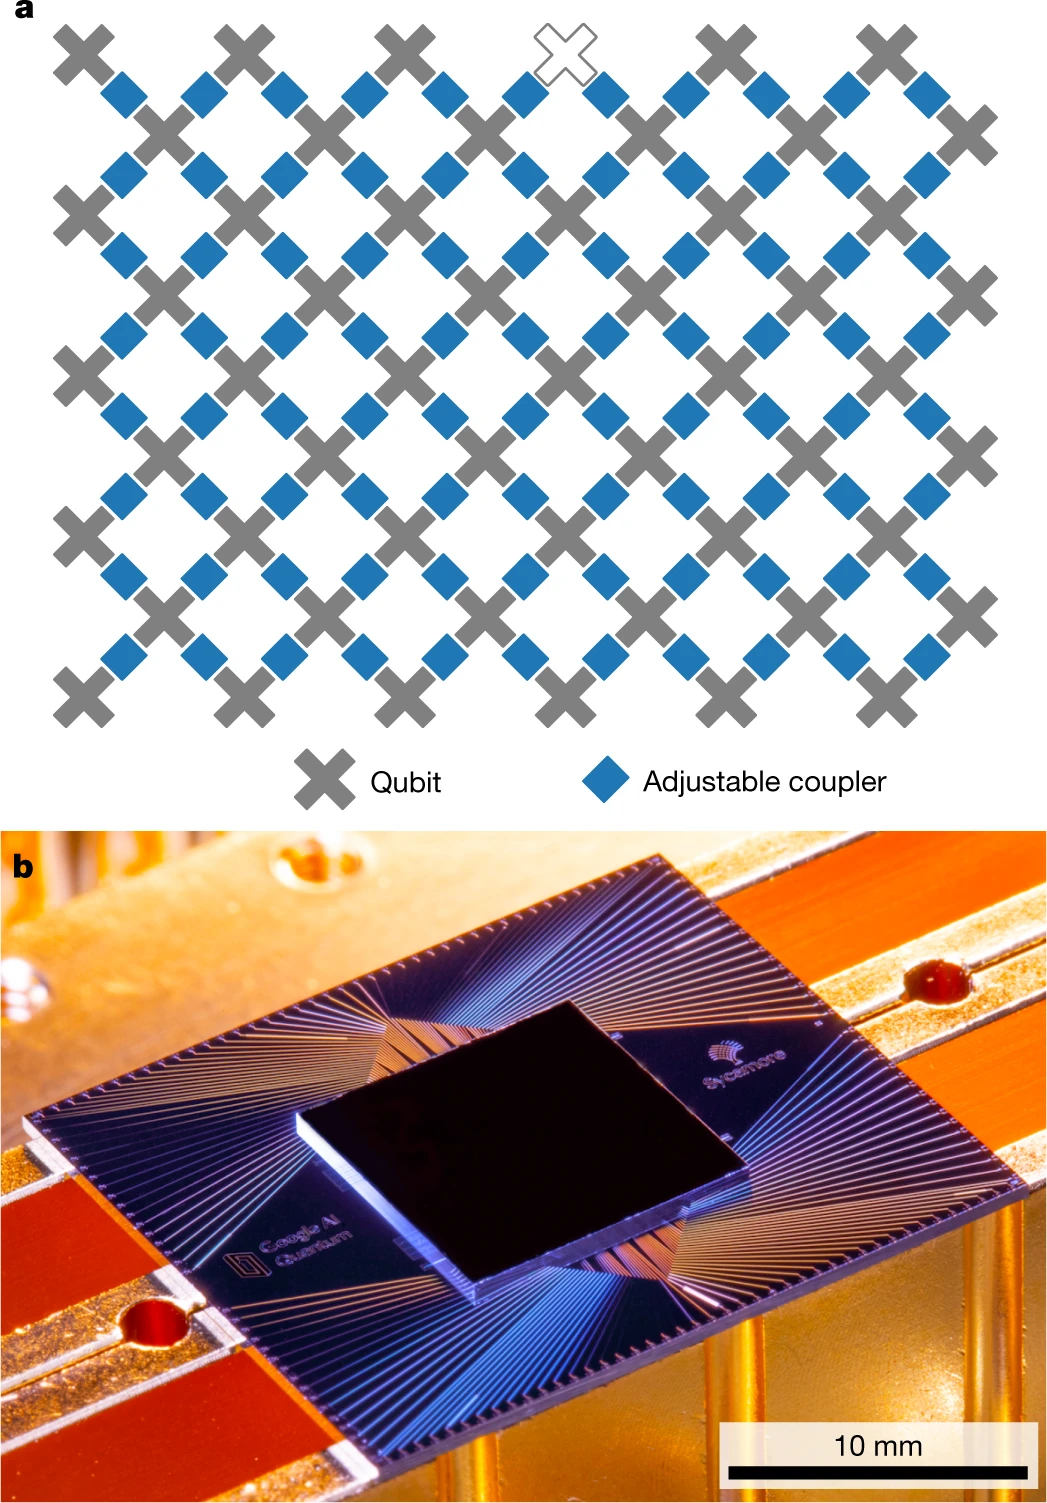
\includegraphics[width=0.7\linewidth]{img/SycamoreChip.png}
    \caption{Sycamore Chip von Google}
    \label{fig:Sycamore}
\end{figure}

\subsubsection{Supraleitende Qubits}
\label{subsub:superleiter}
Quantencomputer mit Supraleitern funktionieren mit elektrischen Schaltkreisen, die bei Temperaturen nahe dem absoluten Nullpunkt betrieben werden. Solche Temperaturen sind nötig,
um die supraleitende Eigenschaft aufrecht zu erhalten.\\

Zwei häufig benutze Qubit-Typen dieser elektrischen Schaltkreise sind:\\
\textbf{Transmon-Qubits}, basiert auf der Ladung des Energieniveaus, welche durch eine Josephson-Junktion kontrolliert wird.\\
\textbf{Flux-Qubits} werden auch durch Josephson-Junktions kontrolliert, beruhen jedoch auf dem magnetischen Fluss in der Schleife.\\

Beide Ansätze basieren auf dem \textbf{Josephson-Effekt}, welcher auftritt, wenn ein supraleitender Strom durch eine dünne Isolierschicht zwischen zwei Supraleitern fließt.\\
Dieser Effekt hat zur Folge, dass eine nichtlineare Spannung-Stom-Beziehung entsteht und für die Manipulation von Qubits genutzt wird.\\

\begin{figure}[H]
    \centering
    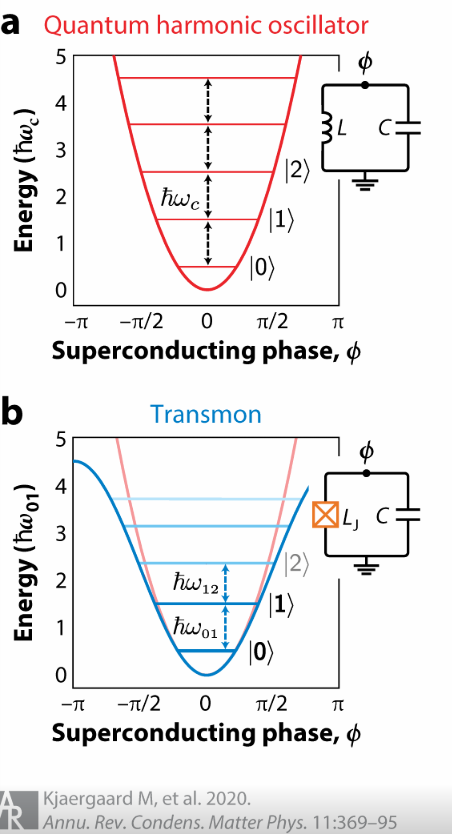
\includegraphics[width=0.75\linewidth]{img/JJ.png}
    \caption{Josephson-Effekt mit einem Josephson Junktion}
    \label{fig:Josephson-junktion}
\end{figure}

In der vorliegenden Abbildung wird der Unterschied zwischen einer harmonischen Quantenschwankung (a) und der nichtlinearen Schwankung des Energie Niveaus der Josephson Junktion (b) abgebildet.\\

Der Phasenunterschied bei der harmonischen Oscellation, gekennzeichnet als $\hbar\omega_c$, ist identisch. Auf der Abbildung ist zu sehen, dass das Energieniveau der Phasen zwischen $\ket{0} \leftrightarrow \ket{1}$
und $\ket{1} \leftrightarrow \ket{2}$ identisch ist und dadurch nicht unterschieden werden kann zwischen welcher Phase gewechselt wurde.\\

Mit einer Josephson Junktion kann jedoch eine nichtlineare Schwankung des Energieniveaus erreicht werden, die auf der Abbildung als orangenes $\boxtimes$ gekennzeichnet ist (b).
Durch diese nichtlineare Schwankung ist das Energie Niveau zwischen den Phasen $\ket{0} \leftrightarrow \ket{1}$ und $\ket{1} \leftrightarrow \ket{2}$ unterschiedlich groß und kann somit unterschieden werden.
Der als $\hbar\omega_{01}$ gekennzeichnete Energieunterschied ist unser Qubit\\

\textbf{Steuerung und Auslesung}\\
Die Steuerung der Josephson-Junktion erfolgt durch Mikrowellenpulse, welche die Energie des Qubits verändern. Die Auslesung erfolgt durch eine Mikrowellenresonanz um die Energie des Qubits zu messen.\\

\subsubsection{Quantenpunkte}
\label{subsub:quantenpunkte}
Quantencomputer basierend auf Quantenpunkten, auch Quantum-Dot genannt, nutzen winzige Halbleiterstrukturen um Qubits zu realisieren.
Quantum-Dots sind künstlich erzeugte Nano-Partikel, in denen Elektronen in drei Dimensionen eingeschlossen sind, was zu quantisierten Einergiezuständen führt.\\

Die Größe eines Quantum-Dots ist typischerweise 2-10 Nanometer und es schließt eine kleine Anzahl oder ein einzelnes Elektron ein.
Für die Fertigung werden oftmals Galliumarsenid (GaAs) oder Silizium (Si) verwendet. Der physikalische Einschluss der Elektronen schränkt ihre
Bewegung stark ein, wodurch ein quantisiertes Energieniveau entsteht. Dies ähnelt dem Energieniveaus eines Atoms, weswegen Quantum-Dots auch als künstliche Atome bezeichnet werden.\\

Die Zustände der Qubits werden durch die Eigenschaften einzelner Elektronen in den Quantum Dots definiert. Es gibt zwei Hauptansätze zur Realisierung von Qubits mit Quantum Dots.\\

\textbf{Ladungs-Qubits}\\
Der Ladungszustand eine Quantum Dots kann als Qubit verwendet werden. Die Ladung eines Elektrons kann entweder 0 oder 1 sein, was als $\ket{0}$ und $\ket{1}$ interpretiert wird.
Für eine Messung wird der Ladungszustand mit einer Kapazitätsmessung der Tunnelströme ermittelt.
Für die Manipulation des Qubits werden elektrische Felder verwendet, um die Elektronen in den Quantum Dots zu bewegen.\\

Diese Methode ist durch die Ladungsquantisierung sehr genau, jedoch auch sehr empfindlich gegenüber Störungen durch die Umgebung.\\

\textbf{Spin-Qubits}\\
Die Spin-Eigenschaften von Elektronen in Quantum Dots können auch als Qubit verwendet werden. Hierbei sind die beiden Spinrichtungen($\uparrow$ für Spin-Up und $\downarrow$ für Spin-Down)
dieser beiden Spinrichtungen entsprechen den Zuständen $\ket{0}$ und $\ket{1}$. Und die Kombination aus beiden Zuständen ergibt eine Superposition.\\

\begin{figure}[H]
    \centering
    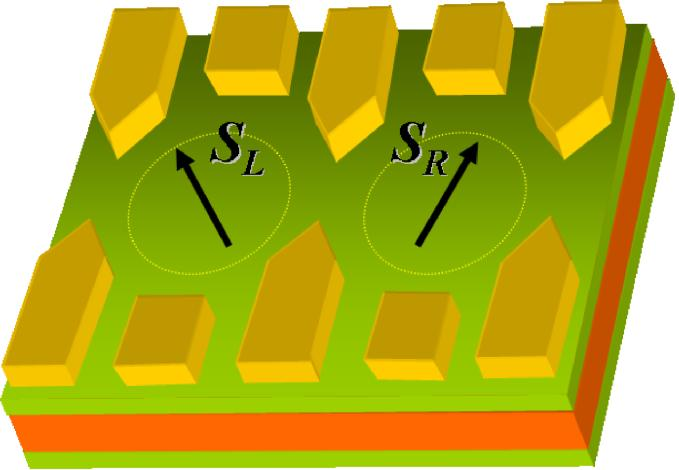
\includegraphics[width=0.75\linewidth]{img/QD.png}
    \caption{Ein doppel Quantum-Dot Qubit}
    \label{fig:double-Quantum-Dot}
\end{figure}

In der Abbildung ist ein Doppel Quantum-Dot Qubit dargestellt. Sowohl in $S_L$ als auch $S_R$ befinden sich Elektornen. Beide können seperat voneinander, sowohl im Spin als auch Ladung, manipuliert werden.
Durch die physikalische Nähe der beiden Quantum-Dots können durch Tunnelkopplung und Austauschwechselwirkung die beiden Qubits miteinander verschränkt werden.\\

Die Umsetzung dieser Methode beschränkt sich hauptsächlich auf die Spin-Variante. Der Grund dafür ist, dass durch die hohe Ladungsanforderung der Ladungsvariante die Qubits sehr empfindlich gegenüber Störungen sind.
Außerdem sind die Nachteile der Spin-Variante gegenüber der Ladungsvariante nicht so gravierend.\\
Jedoch sind die größten Herausforderungen die Herstellung der Halbleiterstrukturen und die Kontrolle der Elektronen in den Quantum-Dots.
Damit ist der größte Vorteil, die hohe Skalierbarkeit, auch der größte Nachteil, da die Herstellung und Kontrolle von vielen Quantum-Dots sehr aufwendig und schwierig ist.\\

\subsubsection{Topologische Quantencomputer}
\label{subsub:topologische_quantencomputer}
Der Ansatz von topologischen Quantencomputern ist völlig anders als die bisher genannten. Im Gegensatz zu verher erläuterten Quantencomputern, welche auf Eigenschaften einzelner Elektronen oder Energieniveaus basieren, basieren topologische Quantencomputer auf topologischen Eigenschaften von Materie.\\
Diese Methode soll das Problem der Dekoheränz minimieren, indem sie Qubits aus Majorana-Partikeln aufbauen.\\

\textbf{Topologie in der Physik}\\
In einem physikalischem System beschreibt die Topologie die Eigenschaften, welche sich nicht durch Deformation verändern lassen.
Ein Beispiel hierfür ist ein Kaffeebecher, der sich durch Verformung in eine Donutform umwandeln lässt. Beide haben die topologische Eigenschaft eines Loches.
Daraus folgernd ist es nicht möglich, einen Kaffeebecher oder ein Donut in eine Kugel zu verformen ohne die topologische Eigenschaft zu verändern.\\

\textbf{Funktionsweise}\\
Die physikalische Grundlage für topologische Quantencomputer liegt in speziellen Materialien und Systemen, die topologische Materiephasen unterstützen.
Ein prominentes Beispiel ist die Verwendung von Majorana-Quasiteilchen, die in bestimmten Supraleitern auftreten können.\\

\begin{figure}[H]
    \centering
    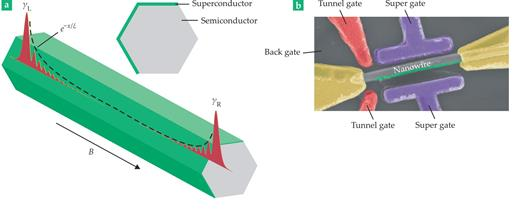
\includegraphics[width=0.75\linewidth]{img/Majorana.png}
    \caption{Nanowire mit Majorana-Quasiteilchen}
    \label{fig:Majorana}
\end{figure}

In der Abbildung ist ein Nanowire dargestellt, der durch ein Supraleiter und ein Magnetfeld in eine topologische Phase gebracht wird.
Diese Art von Partikel treten immer als Paar auf und bilden eine Art Brücke zwischen den Enden des Nanowire und besteht auf einer Vielzahl von Elektronen.
Diese Brücke wird durch die topologischen Eigenschaften der Majorana-Partikel stabilisiert und ist somit weniger anfällig gegenüber Störungen.\\


\begin{tcolorbox}[title=Kommentar,
    title filled=false,
    colback=cyan!5!white,
    colframe=cyan!75!black]
    Die Vertiefung der durch den Quanten-Hall Effekt entsteht wird nur oberflächlich behandelt. Ist jedoch essentiell für die Funktionsweise von Topologischen Quantencomputern.
\end{tcolorbox}

\textbf{Verpflechtung}\\
Braiding ist der Prozess, bei dem die Majorana-Partikel miteinander verflochten werden, um die Quantenbits zu manipulieren. 
Dies passiert auf einer zweidimensionalen Oberfläche, auf der die Majorana-Partikel miteinander verflochten werden.\\

\begin{figure}[H]
    \centering
    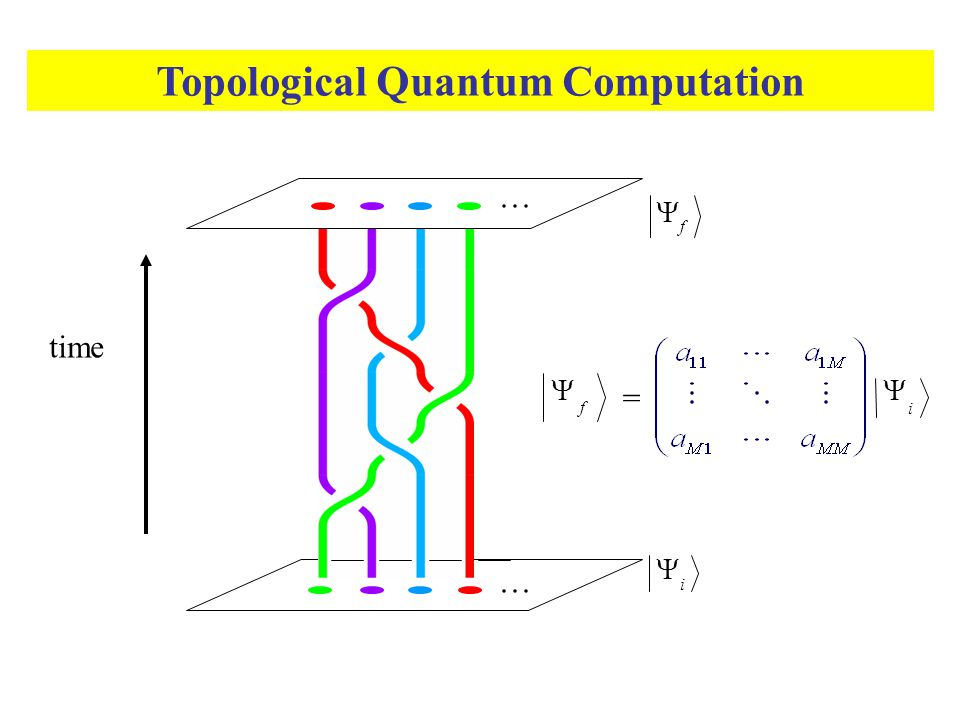
\includegraphics[width=0.75\linewidth]{img/TQC.png}
    \caption{Braiding von Majorana-Quasiteilchen}
    \label{fig:Braiding}
\end{figure}

Hierbei ist die Reihenfolge sehr wichtig, da durch diese Reihenfolge Quantenoperationen realisiert werden.
Jede Verpflechtung entspricht einer Quantenoperation und durch die Kombination von mehreren Verpflechtungen können beliebige Quantenoperationen realisiert werden.\\

Da die Informationen und Quantenoperationen in der Topologie steckt, sind sie gegenüber kleinen Fehlern in der Bewegung/Störungen unempfindlich.\\

\begin{tcolorbox}[title=Kommentar,
    title filled=false,
    colback=cyan!5!white,
    colframe=cyan!75!black]
    Die Technische Umsetzung von topologischen Quantencomputern ist deutlich komplizierter als es in diesem Abschnitt oberflächlich beschrieben ist.\\
    Bisher hat nur Google einen topologischen Quantencomputer vorgestellt, der jedoch noch nicht in der Lage ist, Quantenoperationen durchzuführen.
\end{tcolorbox}

\subsection{Quantum Error Correction}
\label{sub:quantum_error_correction}
Quantum Error Correction, oder auch QEC genannt, ist grundlegend wichtig für die funktionellen Betrieb eines Quantencomputers. Wie bereits in den vorherigen Abschnitten beschrieben,
sind Qubits sehr anfällig gegenüber Dekoheränz und Quantenrauschen.\\

\textbf{Warum ist Fehlerkorrektur notwendig}\\
Es ist unabdingbar, dass eine Fehlerkorrektur in Quantencomputern implementiert wird, da die Fehleranfälligkeit von physischen Qubits durch bessere Herstellung nur einen gewissen Grad an Fehlertoleranz aufbringen kann, welche nicht genug ist.\\

Fehler treten in Quantencomputer durch drei Hauptquellen auf.\\
1. \textbf{Dekoheränz:} Äußere Einflüsse wie Temperaturschwankungen oder elektromagnetische Felder zerstören die koheränten Eigenschaften der Qubits.\\
2. \textbf{Phasen-Flip-Fehler:} Die Phasenwinkel zwischen den Quantenzuständen werden verändert($\ket{0}\rightarrow\ket{0},\ket{1}\rightarrow-\ket{1}$).\\ 
3. \textbf{Bit-Flip-Fehler:} Die Zustände der Qubits werden verändert ($\ket{0}\rightarrow\ket{1},\ket{1}\rightarrow\ket{0}$).\\

Bei der Fehlerkorrektur von Quantencomputern ist jedoch zu beachten, dass diese nicht wie bei herkömmlichen Computern da durch das No-Cloning-Theorem keine Quanteninformationen kopiert werden können.\\

\textbf{Grundprinzip}\\
Quanten-Fehlerkorrektur verwendet \textbf{Redundanz} um Fehler zu detektieren und zu korrigieren, ohne das die eigentliche Quanteninformationen direkt ausgelesen werden.\\

Eine Art der Redundanz ist der Steane-Code, welcher auf 7 Qubits basiert. Dieser Zusammenschluss aus 7 Physischen Qubits bildet ein logisches Qubit,
welches maximal einen Fehler auf einem der 7 Qubits korrigieren kann. Treten jedoch mehrere Fehler auf, kann der Steane-Code diese nicht mehr korrigieren.\\

\begin{figure}[H]
    \centering
    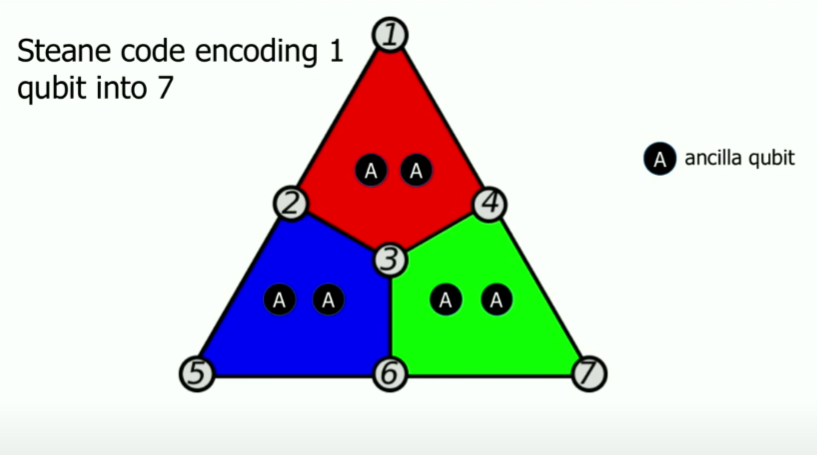
\includegraphics[width=0.75\linewidth]{img/Steane.png}
    \caption{Steane-Code}
    \label{fig:Steane}
\end{figure}

Um die Qubits zu überwachen werden zusätzliche Qubits benötigt, da das direkte Auslesen der daten Qubits den Quantenzustand zerstören würde.
Diese zusätzlichen Qubits werden als \textbf{Ancilla Qubit} bezeichnet und mit den eigentlichen Qubits verschränkt.\\

\textbf{Fehlertoleranz}\\
Diese Herangehensweise ist jedoch auch nicht perfekt. Die Ancilla Qubits sind gleichermaßen anfällig gegenüber Fehlern wie die eigentlichen Qubits.\\

\begin{figure}[H]
    \centering
    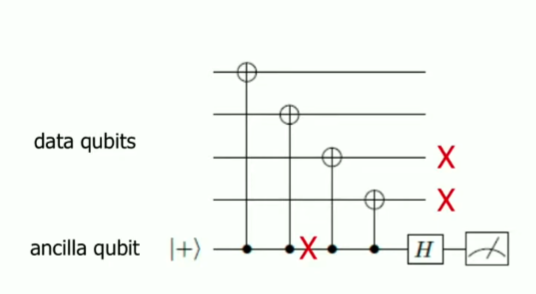
\includegraphics[width=0.75\linewidth]{img/Fehlertoleranz.png}
    \caption{Fehlertoleranz von Ancilla Qubits}
    \label{fig:Fehlertoleranz}
\end{figure}

Dieses Abbildung zeigt, wie ein einzelner Fehler in einem CNOT Gatter auf dem Ancilla Qubit Messung der Daten Qubits als Fehler kennzeichnet, obwohl diese nicht fehlerhaft sind.\\
Die Folge hieraus ist, dass die Fehlerkorrektur mit wenigen Qubits nicht ausreicht um diesen logischen Qubit vollkommen fehlerfrei zu halten.\\

Hierbei werden zwischen zwei Paritätchecks unterschieden. Ein $Z$ und $X$ Parität, welcher festlegt, ob der Fehler in den Ancilla Qubits CNOT Gattern oder den Daten Qubits aufgetreten ist.\\

\textbf{Suface Code}\\
Eine weitere Methode zur Fehlerkorrektur ist der Surface Code, welcher auf einem 2D Gitter von Qubits basiert.
Dieser Code ist in der Lage Fehler zu detektieren und zu korrigieren, solange die Fehlerdichte unter einem bestimmten Wert bleibt.\\

Die Größe des Surface Codes ist variabel und kann skaliert werden, um die Fehlerkorrektur zu verbessern.
Es gibt jedoch ein Threshold, an der die Vergößerung des Codes keine Verbesserung mehr bringt.
Durch die vorher besprochene Fehlertoleranz der Ancilla Qubits wird die Effektivität des Surface Codes gedeckelt.
Die Fehler in der Korrektur werden hierbei mehr, als wenn keine Korrektur vorgenommen wird und es würde keinen Sinn ergeben, den Surface Code weiter zu vergößern.\\

Die Nachfolgende Abbildung eines Surface Codes des Grades $d=3$ zeigt wie die Qubits in einem 2D Gitter angeordnet sind und wie die Fehlerkorrektur durchgeführt wird.
Jede Überschneidung des Gatters stellt ein physischen Qubit dar. Die Kreise in den Quadraten sind die Ancilla Qubits, welche die Fehlerkorrektur durchführen.\\

\begin{figure}[H]
    \centering
    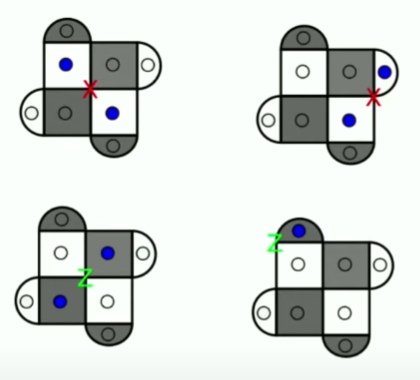
\includegraphics[width=0.6\linewidth]{img/Errors.png}
    \caption{Fehlerkorrektur durch Surface Code des Grades $d=3$}
    \label{fig:Surface-Code}
\end{figure}

Ancilla Qubits in einem weißen Feld prüfen die Qubits auf ein logisches $X$ und Ancilla Qubits in einem Schwarzen Feld prüfen die Qubits auf ein logisches $Z$.\\

Ancilla Qubits, die ein Fehler erkennen, werden als Blau markiert. Durch die Position dieser und für welche Daten Qubits diese zuständig sind wissen wir welche Qubits fehlerhaft sind.\\

\textbf{Praktische Umsetzung}\\
Am 09.12.2024 hat Google den ersten selbst korrigierenden Quantencomputer vorgestellt, der auf dem Surface Code basiert.
Der Chip namens \textbf{Willow} basiert auf 105 physischen Qubits, wobei diese auf der 7x7 Surface Code Architektur aufbaut.
Dies resultiert in 49 Qubits, die deutlich weniger anfällig gegen Fehler sind als phyische Qubits. Die restlichen Qubits werden für Parität und error Korrektur gebraucht.\\

\begin{figure}[H]
    \centering
    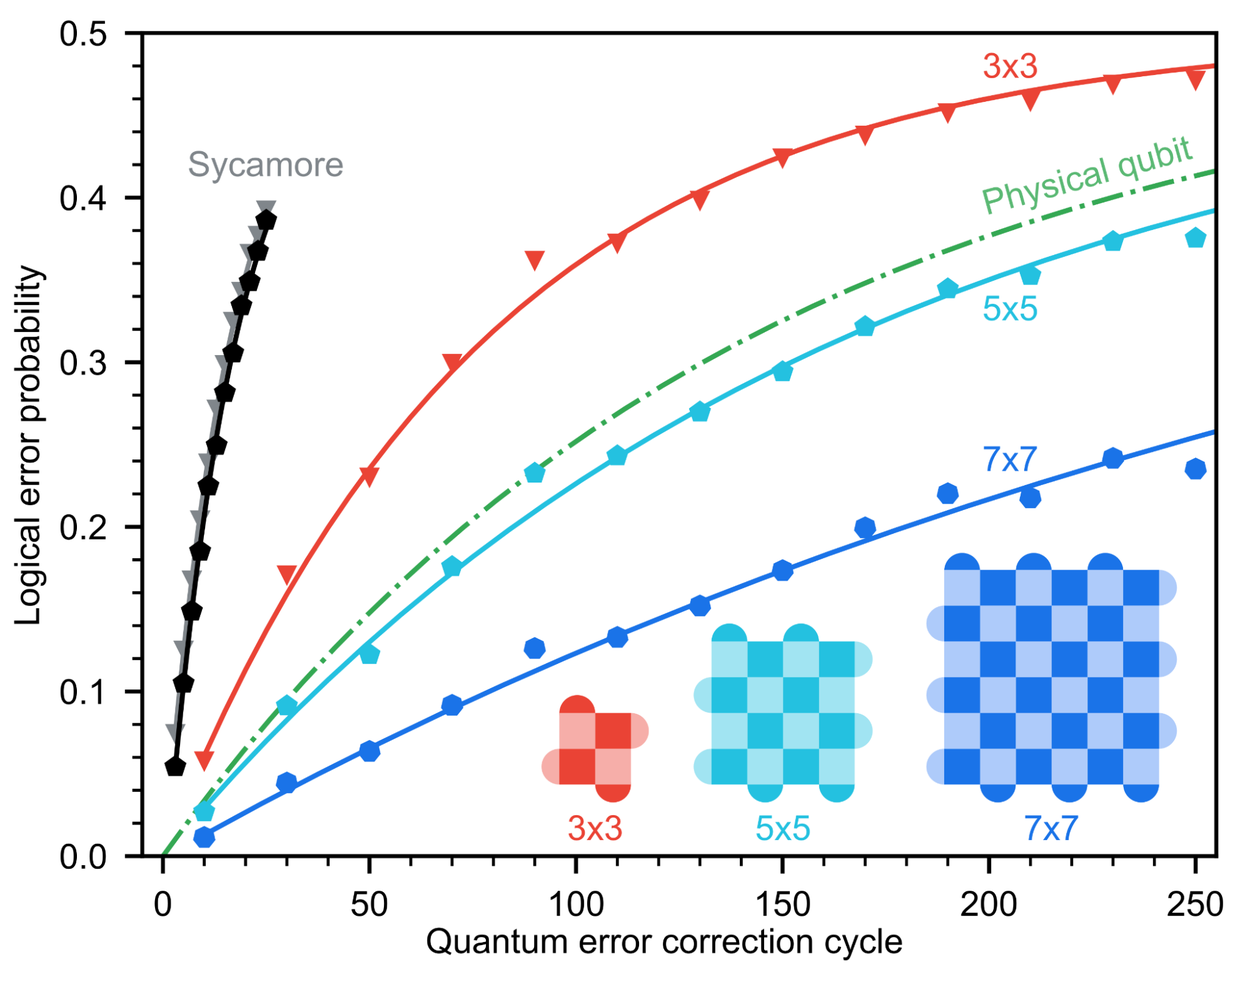
\includegraphics[width=0.7\linewidth]{img/Surface-Code-Scaling.png}
    \caption{Error Korrektur des 7x7 Surface Code}
    \label{fig:Willow}
\end{figure}

Außerdem wurde durch die Anwendung des Surface Codes die $T_1$ Zeit von $20\mu s$ auf $68\mu s\pm13\mu s$ erhöht und ermöglich hierdurch mehr Operationen pro Qubit.\\

\newpage 

\bibliographystyle{natdin}
	\bibliography{references} % expects file "references.bib"
	\addcontentsline{toc}{section}{References}
\end{document}
